% coding:utf-8

%FOSAET, a LaTeX-Code for a electrical summary of basic electronics
%Copyright (C) 2013, Daniel Winz, Ervin Mazlagic

%This program is free software; you can redistribute it and/or
%modify it under the terms of the GNU General Public License
%as published by the Free Software Foundation; either version 2
%of the License, or (at your option) any later version.

%This program is distributed in the hope that it will be useful,
%but WITHOUT ANY WARRANTY; without even the implied warranty of
%MERCHANTABILITY or FITNESS FOR A PARTICULAR PURPOSE.  See the
%GNU General Public License for more details.
%----------------------------------------

\section{Kirchhoffsche Gesetze}

\subsection{Super-Knoten}
Die Kirchhoff'sche Knotenregel besagt, dass die Summer aller Ströme eines Knoten gleich Null ist.
Dieser Zusammenhang kann auch dann genutzt werden wenn keine idealen Knoten vorhanden sind.
Eine Schaltung kann beliebig zu einen Knoten abstrahiert werden und die Knotenströme zu ermitteln.

\begin{figure}[h!]
\centering
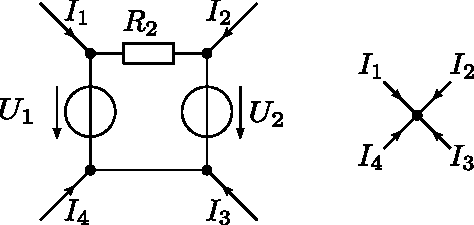
\includegraphics[scale=\schscale]{supernode_sch.pdf}
\caption{Super-Knoten}
\label{sch:supernode}
\end{figure}

\noindent
\textbf{Achtung!} Dieses Prinzip der Zusammenfassung einer Schaltung zu einem Knoten darf nur dazu genutzt werden, um die Ströme in und aus dem Knoten heraus zu ermitteln. Die abstrahierte Schaltung in innern darf jedoch nicht ohne diese Ströme betrachtet werden. 
